\chapter{Dirichlet's Unit Theorem}
In this chapter we will prove Dirichlet's unit theorem, 
which is a structure theorem for the group
of units of the ring of integers of a number field.  The answer is
remarkably simple: if~$K$ has~$r$ real and~$s$ pairs of
complex conjugate embeddings,
then 
$$
\O_K^*\ncisom \Z^{r+s-1} \times T,
$$
where $T$ is a finite cyclic group.

Many questions can be encoded as questions about the structure of the
group of units.  For example, Dirichlet's unit theorem explains
the structure of the  integer solutions $(x,y)$ to Pell's equation $x^2-dy^2=1$
(see Section~\ref{sec:pell}).


\section{The Group of Units}
\begin{definition}[Unit Group]
The \defn{group of units} $U_K$ associated to a number field~$K$ is the
group of elements of $\O_K$ that have an inverse in $\O_K$.
\end{definition}

\begin{theorem}[Dirichlet]\label{thm:units}\ithm{Dirichlet unit}
The group $U_K$ is the product of a finite cyclic group of roots of
unity with a free abelian group of rank $r+s-1$, where~$r$ is the
number of real embeddings of~$K$ and~$s$ is the number of complex
conjugate pairs of embeddings.
\end{theorem}
(Note that we will prove a generalization of Theorem~\ref{thm:units} in
Section~\ref{sec:kummernf} below.)

We prove the theorem by defining a map $\vphi:U_K\to \R^{r+s}$, and
showing that the kernel of $\vphi$ is finite and the image of $\vphi$
is a lattice in a hyperplane in $\R^{r+s}$.  The trickiest part of the
proof is showing that the image of $\vphi$ spans a hyperplane, and we
do this by a clever application of Blichfeld's Lemma~\ref{lem:blichfeld}.

\begin{center}
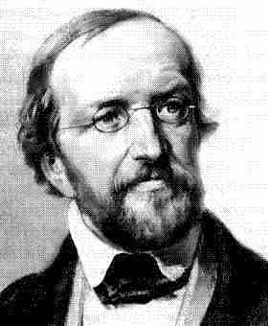
\includegraphics[width=.3\textwidth]{graphics/dirichlet}
%From http://www-gap.dcs.st-and.ac.uk/~history/PictDisplay/Dirichlet.html
\end{center}

\begin{remark}
Theorem~\ref{thm:units} is due to Dirichlet  who lived 1805--1859.
Thomas Hirst described Dirichlet thus:
\begin{quote}He is a rather tall, 
lanky-looking man, with moustache and beard about
to turn grey with a somewhat harsh voice and rather deaf. He was
unwashed, with his cup of coffee and cigar. One of his failings is
forgetting time, he pulls his watch out, finds it past three, and runs
out without even finishing the sentence.
\end{quote}
Koch wrote that:
\begin{quote}
... important parts of mathematics were influenced by Dirichlet. His
proofs characteristically started with surprisingly simple
observations, followed by extremely sharp analysis of the remaining
problem. 
\end{quote}
I think Koch's observation nicely describes the proof we will give of
Theorem~\ref{thm:units}.
\end{remark}



Units have a simple characterization in terms of their norm.
\begin{proposition}\label{prop:unitnorm}\iprop{unit norm characterization}
An element $a\in \O_K$ is a unit if and only if $\Norm_{K/\Q}(a)=\pm 1$.
\end{proposition}
\begin{proof}
Write $\Norm=\Norm_{K/\Q}$.  If $a$ is a unit, then $a^{-1}$ is also a
unit, and $1=\Norm(a)\Norm(a^{-1})$.  Since both $\Norm(a)$ and
$\Norm(a^{-1})$ are integers, it follows that $\Norm(a)=\pm 1$.
Conversely, if $a\in \O_K$ and $\Norm(a)=\pm 1$, then the equation
$aa^{-1}=1=\pm \Norm(a)$ implies that $a^{-1} = \pm \Norm(a)/a$.  But
$\Norm(a)$ is the product of the images of~$a$ in $\C$ by all
embeddings of~$K$ into~$\C$, so $\Norm(a)/a$ is also a product of
images of~$a$ in~$\C$, hence a product of algebraic integers,
hence an algebraic integer.  Thus $a^{-1}\in K\cap \Zbar = \O_K$, 
which proves that~$a$ is a unit.
\end{proof}

\begin{remark}
Proposition~\ref{prop:unitnorm} is false if we replace $\O_K$ by $K$.
For example, if $\alpha$ is a root of $x^2-\frac{1}{2}x+1$, then
$\alpha$ has norm $\pm 1$, but $\alpha$ is not a unit of $\O_K$, since
$\alpha\not\in \O_K$.  To general Proposition~\ref{prop:unitnorm} to an
arbitrary finite extension $R/S$ of Dedekind domains, we replace $\pm
1$ by ``an element of $S^*$''.
\end{remark}

Let $r$ be the number of real and $s$ the number of complex conjugate
embeddings of $K$ into $\C$, so $n=[K:\Q]=r+2s$.
Define the {\em log map}
$$
\vphi:U_K \to \R^{r+s}
$$
by 
$$
 \vphi(a) = (\log|\sigma_1(a)|,\ldots, \log|\sigma_{r+s}(a)|).
$$
(Here $|z|$ is the usual absolute value of $z=x+iy\in\C$, 
so $|z|=\sqrt{x^2+y^2}$.)

\begin{lemma}\label{lem:inh}\ilem{hyperplane embedding}
The image of $\vphi$ lies in the hyperplane 
\begin{equation}\label{eqn:hyperplane}
H = \{(x_1,\ldots, x_{r+s})\in\R^{r+s} : 
  x_1+ \cdots + x_r + 2x_{r+1} + \cdots + 2x_{r+s} = 0\}.
\end{equation}
\end{lemma}
\begin{proof}
If $a\in U_K$, then 
by Proposition~\ref{prop:unitnorm}, 
$$\left(\prod_{i=1}^{r} |\sigma_i(a)|\right) 
  \cdot \left( \prod_{i=r+1}^{r+s} |\sigma_i(a)|^2 \right) = 
|\Norm_{K/\Q}(a)| = 1.$$
Taking logs of both sides proves the lemma.
\end{proof}

\begin{lemma}\label{lem:vphifinitekernel}
The kernel of $\vphi$ is finite.
\end{lemma}
\begin{proof}
We have
\begin{align*}
  \Ker(\vphi) &\subset \{a\in\O_K : |\sigma_i(a)| = 1 \text{ for }i=1,\ldots,r+s\}\\
              &\subset \sigma(\O_K) \cap X,
\end{align*}
where $X$ is the bounded subset of $\R^{r+s}$ of elements all of whose coordinates
have absolute value at most $1$.  Since $\sigma(\O_K)$ is a lattice 
(see Proposition~\ref{prop:ok_lattice}), 
the intersection $\sigma(\O_K)\cap X$ is finite, so $\Ker(\vphi)$ is finite.
\end{proof}

\begin{lemma}\label{lem:kerfcg}
The kernel of~$\vphi$ is a finite cyclic group.
\end{lemma}
\begin{proof}
  Lemma~\ref{lem:vphifinitekernel} implies that $\ker(\vphi)$ is a
  finite group.  It is a general fact that any finite subgroup $G$ of
  the multiplicative group $K^*$ of a field is cyclic.  (Proof: If~$n$
  is the exponent of~$G$, then every element of~$G$ is a root of the
  polynomial $x^n-1$.  A polynomial of degree~$n$ over a field has at
  most~$n$ roots, so $G$ has order at most~$n$, hence~$G$ is cyclic of
  order~$n$.)
\end{proof}

To prove Theorem~\ref{thm:units}, it suffices to prove that
$\Im(\vphi)$ is a lattice in the hyperplane~$H$ of
(\ref{eqn:hyperplane}), which we view as a vector space of dimension
$r+s-1$.

Define an embedding
\begin{equation}\label{eqn:sigma3}
 \sigma : K\hra \R^n
\end{equation}
given by $\sigma(x) = (\sigma_1(x),\ldots,\sigma_{r+s}(x))$,
where we view $\C\isom \R\times \R$ via $a+b i\mapsto (a,b)$.
Thus this is the embedding
\begin{align*}
 x\mapsto \big(&\sigma_1(x), \sigma_2(x),\ldots, \sigma_r(x),\\
     &\quad \Re(\sigma_{r+1}(x)), \Im(\sigma_{r+1}(x)), 
    \ldots, \Re(\sigma_{r+s}(x)), \Im(\sigma_{r+s}(x))\big).
\end{align*}

\begin{lemma}\label{lem:ukdiscrete}
The image $\vphi:U_K\to \R^{r+s}$ is discrete.
\end{lemma}
\begin{proof}
Let $X$ be a bounded subset of $\R^{r+s}$.
We will show that the intersection $\vphi(U_K)\cap X$ is finite.
Since $X$ is bounded, for any $u\in
Y=\vphi^{-1}(X)\subset U_K$ the coordinates of $\sigma(u)$ are bounded, 
since $|\log(x)|$ is bounded on bounded subsets
of $[1,\infty)$.
Thus $\sigma(Y)$ is
a bounded subset of $\R^n$.  Since $\sigma(Y)\subset \sigma(\O_K)$,
and $\sigma(\O_K)$ is a lattice in $\R^n$, it follows that $\sigma(Y)$
is finite; moreover,~$\sigma$ is injective, so $Y$ is finite.
Thus $\vphi(U_K)\cap X \subset \vphi(Y) \cap X$ is finite.
\end{proof}

We will use the following lemma in our
proof of Theorem~\ref{thm:units}.
\begin{lemma}\label{lem:chooseci}
Let $n\geq 2$ be an integer, suppose $w_1,\ldots, w_n\in\R$
are not all equal, and suppose $A, B\in\R$ are positive. Then
there exist $d_1,\ldots, d_{n} \in \R_{>0}$ such that 
$$|w_1\log(d_1)+\cdots +w_{n}\log(d_{n})| > B$$  
and $d_1\cdots d_n = A$.
\end{lemma}
\begin{proof}
Order the $w_i$ so
that $w_1\neq 0$.  By hypothesis there exists a $w_j$ such that
$w_j\neq w_1$, and again re-ordering we may assume that $j=2$.  Set
$d_3=\cdots=d_{r+s}=1$.  Suppose $d_1, d_2$ are any positive real numbers
with  $d_1 d_2 = A$.  Since $\log(1)=0$,
\begin{align*}
  \left|\sum_{i=1}^{n} w_i \log(d_i)\right|
  &= |w_1\log(d_1) + w_2\log(d_2)|\\
  &= |w_1 \log(d_1) + w_2\log(A/d_1)| \\
  &= |(w_1-w_2)\log(d_1) + w_2\log(A)|
\end{align*}
Since $w_1\neq w_2$,  we have $|(w_1-w_2)\log(d_1) + w_2\log(A)|\to\infty$
as $d_1\to \infty$.  It is thus possible to choose the $d_i$ as in the lemma.
\end{proof}

\begin{proof}[Proof of Theorem~\ref{thm:units}]
By Lemma~\ref{lem:ukdiscrete}, the image $\vphi(U_K)$
is discrete, so it remains to show that $\vphi(U_K)$
spans~$H$.  
Let~$W$ be the $\R$-span of the image
$\vphi(U_K)$, and note that~$W$ is a subspace of~$H$,
by Lemma~\ref{lem:inh}.  We will show
that $W=H$ indirectly by showing that if $v\not \in H^{\perp}$,
where~$\perp$ is the orthogonal complement 
with respect to the dot product on $\R^{r+s}$, then
$v\not \in W^{\perp}$.  This will show that $W^{\perp}\subset
H^{\perp}$, hence that $H\subset W$, as required.

Thus suppose $z=(z_1,\ldots,z_{r+s})\not\in H^{\perp}$.  
Define a function $f:K^*\to \R$ by 
\begin{equation}\label{eqn:f}
  f(x) = z_1\log|\sigma_1(x)| + \cdots + z_{r+s}\log|\sigma_{r+s}(x)|.
\end{equation}
Note that $f(U_K)=\{0\}$ if and only if $z\in W^{\perp}$,
so to show that $z\not\in W^{\perp}$ we show that there exists some $u\in
U_K$ with $f(u)\neq 0$.

Let 
$$
  A=\sqrt{|d_K|} \cdot \left( \frac{2}{\pi}\right)^s \in \R_{>0}.
$$
Choose any positive real numbers $c_1,\ldots, c_{r+s} \in \R_{>0}$
such that
$$
  c_1\cdots c_r\cdot (c_{r+1}\cdots c_{r+s})^2 = A.
$$
Let 
\begin{align*}
  S &= \{(x_1,\ldots,x_n) \in \R^n : \\
    &\qquad\qquad |x_i|\leq c_i\text{ for } 1\leq i \leq r,\\
    &\qquad\qquad |x_i^2 + x_{i+s}^2| \leq c_i^2 \text{ for } r<i\leq r+s\} \subset \R^n.
\end{align*}
Then~$S$ is closed, bounded, convex, symmetric with respect to the
origin, and of dimension $r+2s$, since $S$ is a product of~$r$ intervals
and~$s$ discs, each of which has these properties.
Viewing $S$ as a product of intervals and discs, we see that the volume of $S$ is
$$
  \Vol(S) = \prod_{i=1}^r (2c_i) \cdot \prod_{i=1}^s (\pi c_i^2) 
          = 2^r\cdot \pi^s \cdot A
  = 2^{r+s}\sqrt{|d_K|} = 2^n \cdot 2^{-s}\sqrt{|d_K|}.
$$

Recall Blichfeldt's Lemma~\ref{lem:blichfeld}, which asserts  
that if~$L$ is a lattice and~$S$ is closed,
bounded, etc., and has volume at least $2^n\cdot \Vol(V/L)$, then
$S\cap L$ contains a nonzero element.   To apply this lemma, we
take $L=\sigma(\O_K)\subset \R^n$, where $\sigma$ is as in (\ref{eqn:sigma3}).
By Lemma~\ref{lem:volok}, 
we have
$\Vol(\R^n/L) = 2^{-s}\sqrt{|d_K|}$.  To check the hypothesis
of Blichfeld's lemma, note that 
$$
 \Vol(S) = 2^n \cdot 2^{-s} \sqrt{|d_K|} = 2^n \Vol(\R^n/L).
$$
Thus there exists a nonzero element $x$ in $S\cap \sigma(\O_K)$.
Let $a\in \O_K$ with $\sigma(a)=x$, then $\sigma(a)\in S$, so
$|\sigma_i(a)|\leq c_i$ for $1\leq i\leq r+s$.
We then have
\begin{align*}
  |\Norm_{K/\Q}(a)| &=
   \left|\prod_{i=1}^{r+2s} \sigma_i(a)\right|\\
   &=  \prod_{i=1}^r |\sigma_i(a)|\cdot \prod_{i=r+1}^s|\sigma_i(a)|^2\\
   &\leq c_1\cdots c_r\cdot (c_{r+1}\cdots c_{r+s})^2 = A.
\end{align*}
Since $a\in \O_K$ is nonzero, we also have
$$
 |\Norm_{K/\Q}(a)|\geq 1.
$$
Moreover, if for any $i\leq r$, we have $|\sigma_i(a)|< \frac{c_i}{A}$, then 
$$
 1\leq |\Norm_{K/\Q}(a)| < c_1\cdots \frac{c_i}{A}\cdots c_r \cdot (c_{r+1}\cdots c_{r+s})^2 = \frac{A}{A} = 1,
$$
a contradiction, so $|\sigma_i(a)|\geq \frac{c_i}{A}$ for $i=1,\ldots, r$. Likewise,
$|\sigma_i(a)|^2 \geq \frac{c_i^2}{A}$, for $i=r+1,\ldots, r+s$. 
Rewriting this 
we have 
\begin{equation}\label{eqn:cisigbound}
  \frac{c_i}{|\sigma_i(a)|}\leq A\quad\text{ for }i\leq r\quad\text{and}\quad
\left(\frac{c_i}{|\sigma_i(a)|}\right)^2\leq A\quad\text{for } i=r+1,\ldots, r+s.
\end{equation}

Recall that our overall strategy is to use an appropriately chosen~$a$
to construct a unit $u\in U_K$ such $f(u)\neq 0$.  First, let
$b_1,\ldots, b_m$ be representative generators for the finitely many
nonzero principal ideals of $\O_K$ of norm at most $A$.  Since
$|\Norm_{K/\Q}(a)|\leq A$, we have $(a)=(b_j)$, for some $j$, so there
is a unit~$u\in \O_K$ such that $a=u b_j$.

Let 
$$
t = t_{c_1,\ldots, c_{r+s}} = z_1\log(c_1)+\cdots +z_{r+s}\log(c_{r+s}),
$$ 
and recall $f:K^*\to \R$ defined in
(\ref{eqn:f}) above.
We have
\begin{align*}
  |f(u) - t| &= |f(a) - f(b_j) - t|\\
   &\leq |f(b_j)| + |t - f(a)|\\
   &=|f(b_j)| + |z_1(\log(c_1) - \log(|\sigma_1(a)|)) + \cdots + z_{r+s}(\log(c_{r+s}) - \log(|\sigma_{r+s}(a)|))|\\
   &=|f(b_j)| + |z_1\cdot \log(c_1/|\sigma_1(a)|) + \cdots + \frac{z_{r+s}}{2}\cdot \log((c_{r+s}/|\sigma_{r+s}(a)|)^2)|\\
   &\leq |f(b_j)| + \log(A)\cdot\left(\sum_{i=1}^{r}|z_i| + \frac{1}{2}\cdot \sum_{i=r+1}^s|z_i|\right) \defeq B_j.
\end{align*}
In the last step we use (\ref{eqn:cisigbound}).

Let $B=\max_{j} B_j$, and note that $B$ does not depend on the choice
of the $c_i$; in fact, it only depends our {\em fixed} choice of $z$ and on the field $K$.
Moreover, for any choice of the $c_i$ as above, we have
$$
  |f(u) - t| \leq B.
$$
If we can choose positive real numbers~$c_i$ such that
\begin{align*}
 c_1\cdots c_r\cdot (c_{r+1}\cdots c_{r+s})^2 &= A\\
  |t_{c_1,\ldots, c_{r+s}}| &>B,
\end{align*}
then the fact that $|f(u)-t|\leq B$ would then imply that $|f(u)|>0$,
which is exactly what we aimed to prove.

If $r+s=1$, then we are trying to prove that $\vphi(U_K)$ is a lattice
in $\R^0=\R^{r+s-1}$, which is automatically true, so assume $r+s>1$.
To finish the proof, we explain how to use Lemma~\ref{lem:chooseci}
to choose $c_i$ such that $|t|>B$.  We have
\begin{align*}
t &= z_1\log(c_1)+\cdots +z_{r+s}\log(c_{r+s})\\
&= z_1\log(c_1)+\cdots +  z_r\log(c_r)+
\frac{1}{2}\cdot z_{r+1}\log(c_{r+1}^2) + 
\cdots + \frac{1}{2}\cdot z_{r+s}\log(c_{r+s}^2)\\
&=w_1\log(d_1)+\cdots +  w_r\log(d_r)+
w_{r+1}\log(d_{r+1}) + 
\cdots +\cdot w_{r+s}\log(d_{r+s}),
\end{align*}
where $w_i=z_i$ and $d_i=c_i$ for $i\leq r$, and
$w_i=\frac{1}{2}z_i$ and $d_i=c_i^2$ for $r<i\leq r+s$.
The condition that $z\not\in H^{\perp}$ is that the $w_i$ are not all
the same, 
 and in our new coordinates the lemma is equivalent to
showing that $|\sum_{i=1}^{r+s} w_i \log(d_i)|>B$, subject to the
condition that $\prod_{i=1}^{r+s} d_i = A$. 
But this is exactly what Lemma~\ref{lem:chooseci} shows.
It is thus possible
to find a unit~$u$ such that $|f(u)|>0$.  Thus $z\not\in
W^{\perp}$, so $W^{\perp}\subset H^{\perp}$, whence $H\subset W$,
which finishes the proof of Theorem~\ref{thm:units}.
\end{proof}

\section{Examples with Sage}
\subsection{Pell's Equation}\label{sec:pell}
The so-called ``Pell's equation'' is $x^2-dy^2 = 1$ with $d>0$ square
free, and we seek integer solutions $x,y$ to this equation.  If
$x+y\sqrt{d}\in K = \Q(\sqrt{d})$, then
$$
  \Norm(x+y\sqrt{d}) = (x+y\sqrt{d})(x-y\sqrt{d}) = x^2 -dy^2.
$$ 
Thus if $(x,y)$ are integers such that $x^2 - d y^2 = 1$, then $\alpha
= x + \sqrt{d}y \in \O_K$ has norm $1$, so by
Proposition~\ref{prop:unitnorm} we have $\alpha \in U_K$.  The integer
solutions to Pell's equation thus form a finite-index subgroup of the
group of units in the ring of integers of $\Q(\sqrt{d})$.  Dirichlet's
unit theorem implies that for any~$d$ the solutions to Pell's equation
with $x,y$ not both negative forms an infinite cyclic group, which is
a fact that takes substantial work to prove using only elementary
number theory (for example, using continued fractions).

We first solve Pell's equation $x^2 - 5y^2 = 1$ with $d=5$ by finding
the units of the ring of integers of $\QQ(\sqrt{5})$ using Sage.

\begin{lstlisting}
sage: K.<sqrt5> = QuadraticField(5)
sage: G = K.unit_group(); G
Unit group with structure C2 x Z of Number Field in sqrt5 with 
defining polynomial x^2 - 5
sage: G.0
-1
sage: u = G.1; u
1/2*sqrt5 - 1/2
\end{lstlisting}

The subgroup of cubes gives us the units with integer $x,y$ (not both negative).

\begin{lstlisting}
sage: u, u^2, u^3, u^4, u^5, u^6
(1/2*sqrt5 - 1/2, -1/2*sqrt5 + 3/2, sqrt5 - 2, -3/2*sqrt5 + 7/2, 
 5/2*sqrt5 - 11/2, -4*sqrt5 + 9)
sage: [list(v^i) for i in [0..9]]
[[1, 0], [-2, 1], [9, -4], [-38, 17], [161, -72], [-682, 305], [2889, 
 -1292], [-12238, 5473], [51841, -23184], [-219602, 98209]]
\end{lstlisting}

% \begin{verbatim}
%    > R<x> := PolynomialRing(RationalField());
%    > K<a> := NumberField(x^2-5);
%    > G, phi := UnitGroup(K);
%    > G;
%    Abelian Group isomorphic to Z/2 + Z
%    Defined on 2 generators
%    Relations:
%        2*G.1 = 0
%    > K!phi(G.1);
%    -1
%    > u := K!phi(G.2); u;
%    1/2*(a + 1)
%    > u^2;
%    1/2*(a + 3)
%    > u^3;
%    a + 2
%    > Norm(u);
%    -1
%    > Norm(u^3);
%    -1
%    > Norm(u^6);
%    1
%    > fund := u^6;
%    > fund;
%    4*a + 9
%    > 9^2 - 5*4^2;
%    1
%    > fund^2;
%    72*a + 161
%    > fund^3;
%    1292*a + 2889
%    > fund^4;
%    23184*a + 51841
%    > fund^5;
%    416020*a + 930249
% \end{verbatim}

A great article about Pell's equation is \cite{lenstra:pell}.  The
MathSciNet review begins: ``This wonderful article begins with history
and some elementary facts and proceeds to greater and greater depth
about the existence of solutions to Pell equations and then later the
algorithmic issues of finding those solutions. The cattle problem is
discussed, as are modern smooth number methods for solving Pell
equations and the algorithmic issues of representing very large
solutions in a reasonable way.''

The simplest solutions to Pell's equation can be huge, even when~$d$
is quite small.  Read Lenstra's paper for some examples from
over two thousand years ago.  Here is one example for $d=10000019$.

\begin{lstlisting}
sage: K.<a> = QuadraticField(next_prime(10^7))
sage: G = K.unit_group(); G.1
163580259880346328225592238121094625499142677693142915506747253000
340064100365767872890438816249271266423998175030309436575610631639
272377601680603795883791477817611974184075445702823789975945910042
8895693238165048098039*a - 
517286692885814967470170672368346798303629034373575202975075605058
714958080893991274427903448098643836512878351227856269086856679078
304979321047765031073345259902622712059164969008633603603640331175
6634562204182936222240930
\end{lstlisting}

\begin{exercise}
  Let $U$ be the group of units $x+y\sqrt{5}$ of the ring of integers
  of $K=\QQ(\sqrt{5})$.  
\begin{enumerate}
\item Prove that the set $S$ of units $x+y\sqrt{5} \in U$ with
  $x,y\in\ZZ$ is a subgroup of $U$.  (The main point is to show that
  the inverse of a unit with $x,y\in\Z$ again has coefficients in
  $\Z$.)
\item Let $U^3$ denote the subgroup of cubes of elements of $U$.
  Prove that $S=U^3$ by showing that $U^3\subset S \subsetneq U$ and
  that there are no groups $H$ with $U^3\subsetneq H \subsetneq U$.
\end{enumerate}
\end{exercise}

\subsection{Examples with Various Signatures}
In this section we give examples for various $(r,s)$ pairs. 
First we consider $K=\Q(i)$.
\begin{lstlisting}
sage: K.<a> = QuadraticField(-1)
sage: K.signature()
(0, 1)
sage: U = K.unit_group(); U
Unit group with structure C4 of Number Field in a with 
defining polynomial x^2 + 1
sage: U.0
-a
\end{lstlisting}

%    > R<x> := PolynomialRing(RationalField());
%    > K<a> := NumberField(x^2+1);
%    > Signature(K);
%    0 1    // r=0, s=1
%    > G,phi := UnitGroup(K);
%    > G;
%    Abelian Group isomorphic to Z/4
%    Defined on 1 generator
%    Relations:
%        4*G.1 = 0
%    > K!phi(G.1);
%    -a


The {\tt signature} method returns the
number of real and complex conjugate embeddings
of $K$ into $\C$.  The \verb|unit_group| method,
which we used above, returns the unit group $U_K$
as an abstract abelian group and a homomorphism $U_K\to \O_K$.

Next we consider $K=\Q(\sqrt[3]{2})$.
\begin{lstlisting}
sage: R.<x> = QQ[]
sage: K.<a> = NumberField(x^3 - 2)
sage: K.signature()
(1, 1)
sage: U = K.unit_group(); U
Unit group with structure C2 x Z of Number Field in a with 
defining polynomial x^3 - 2
sage: U.gens()
[-1, a - 1]
sage: u = U.1; u
a - 1
\end{lstlisting}

%    > K<a> := NumberField(x^3-2);
%    > Signature(K);
%    1 1
%    > G,phi := UnitGroup(K);
%    > G;
%    Abelian Group isomorphic to Z/2 + Z
%    Defined on 2 generators
%    Relations:
%        2*G.1 = 0
%    > K!phi(G.2);
%    -a + 1


Below we use the \verb|places| command, which returns the real embeddings
and representatives for the complex conjugate embeddings.
We use the places to define the log map $\varphi$, which plays such a big
role in this chapter. 
\begin{lstlisting}
sage: S = K.places(prec=53); S
[Ring morphism:
  From: Number Field in a with defining polynomial x^3 - 2
  To:   Real Double Field
  Defn: a |--> 1.25992104989, Ring morphism:
  From: Number Field in a with defining polynomial x^3 - 2
  To:   Complex Double Field
  Defn: a |--> -0.629960524947 + 1.09112363597*I]
sage: phi = lambda z : [log(abs(sigma(z))) for sigma in S]
sage: phi(u)
[-1.34737734833, 0.673688674165]
sage: phi(K(-1))
[0.0, 0.0]
\end{lstlisting}
Note that $\vphi:U_K \to \R^2$, and the image lands in the
1-dimensional subspace of $(x_1,x_2)$ such that $x_1 +2x_2 = 0$. Also,
note that $\varphi(-1)=0$.

%    > Conjugates(K!phi(G.2));
%    [ -0.25992104989487316476721060727822835057025146470099999999995,
%    1.6299605249474365823836053036391141752851257323513843923104 - 
%    1.09112363597172140356007261418980888132587333874018547370560*i, 
%    1.6299605249474365823836053036391141752851257323513843923104 + 
%    1.09112363597172140356007261418980888132587333874018547370560*i ]
%    > Logs(K!phi(G.2));   // image of infinite order unit -- generates a lattice
%    [ -1.34737734832938410091818789144565304628306227332099999999989\
%    , 0.6736886741646920504590939457228265231415311366603288999999 ]
%    > Logs(K!phi(G.1));   // image of -1
%    [ 0.E-57, 0.E-57 ]

Let's try a field such that $r+s-1=2$.  First, one with $r=0$ and
$s=3$:
\begin{lstlisting}
sage: K.<a> = NumberField(x^6 + x + 1)
sage: K.signature()
(0, 3)
sage: U = K.unit_group(); U
Unit group with structure C2 x Z x Z of Number Field in a with 
defining polynomial x^6 + x + 1
sage: u1 = U.1; u1
a
sage: u2 = U.2; u2
a^3 + a
sage: S = K.places(prec=53)
sage: phi = lambda z : [log(abs(sigma(z))) for sigma in S]
sage: phi(u1)
[-0.167415483286, 0.0486439097527, 0.118771573533]
sage: phi(u2)
[0.306785708923, -1.07251465055, 0.765728941626]
sage: phi(K(-1))
[0.0, 0.0, 0.0]
sage: sum(phi(u1))
-2.63677968348e-15
sage: sum(phi(u2))
-5.10702591328e-15
\end{lstlisting}
%    > K<a> := NumberField(x^6+x+1);
%    > Signature(K);
%    0 3
%    > G, phi := UnitGroup(K);
%    > G;
%    Abelian Group isomorphic to Z/2 + Z + Z
%    Defined on 3 generators
%    Relations:
%        2*G.1 = 0
%    > u1 := K!phi(G.2); u1;
%    a
%    > u2 := K!phi(G.3); u2;
%    -2*a^5 - a^3 + a^2 + a
%    > Logs(u1);
%    [ 0.11877157353322375762475480482285510811783185904379239999998, 
%    0.048643909752673399635150940533329986148342128393119899999997, 
%    -0.16741548328589715725990574535618509426617398743691229999999 ]
%    > Logs(u2);
%    [ 1.6502294567845884711894772749682228152154948421589999999997, 
%    -2.09638539134527779532491660083370951943382108902299999999997, 
%    0.44615593456068932413543932586548670421832624686433469999994 ]

Notice that the log image of $u_1$ is clearly not a real multiple of
the log image of~$u_2$ (e.g., the scalar would have to be positive
because of the first coefficient, but negative because of the second).
This illustrates the fact that the log images of $u_1$ and $u_2$ span
a two-dimensional space.

Next we compute a field with $r=3$ and $s=0$.  (A field with $s=0$
is called totally real.)
\begin{lstlisting}
sage: K.<a> = NumberField(x^3 + x^2 - 5*x - 1)
sage: K.signature()
(3, 0)
sage: U = K.unit_group(); U
Unit group with structure C2 x Z x Z of Number Field in a with 
defining polynomial x^3 + x^2 - 5*x - 1
sage: u1 = U.1; u
a - 1
sage: u2 = U.2; u2
a
sage: S = K.places(prec=53)
sage: phi = lambda z : [log(abs(sigma(z))) for sigma in S]
sage: phi(u1)
[-0.774767022346, -0.392848724581, 1.16761574693]
sage: phi(u2)
[0.996681204093, -1.64022415032, 0.643542946229]
\end{lstlisting}

%    > K<a> := NumberField(x^3 + x^2 - 5*x - 1);
%    > Signature(K);
%    3 0
%    > G, phi := UnitGroup(K);
%    > G;
%    Abelian Group isomorphic to Z/2 + Z + Z
%    Defined on 3 generators
%    Relations:
%        2*G.1 = 0
%    > u1 := K!phi(G.2); u1;
%    1/2*(a^2 + 2*a - 1)
%    > u2 := K!phi(G.3); u2;
%    a
%    > Logs(u1);
%    [ 1.16761574692758757159598251863681302946987760474899999999995, 
%    -0.39284872458139826129179862583435951875841422643044369999996, 
%    -0.7747670223461893103041838928024535107114633783181766999998 ]
%    > Logs(u2);
%    [ 0.6435429462288618773851817227686467257757954024463081999999, 
%    -1.6402241503223171469101505551700850575583464226669999999999, 
%    0.9966812040934552695249688324014383317825510202205498999998 ]

A field with $r=0$ is called totally complex.  For
example, the \defn{cyclotomic fields} $\Q(\zeta_n)$ are totally
complex, where $\zeta_n$ is a primitive $n$th root of 
unity.  The degree of $\Q(\zeta_n)$ over $\Q$ is
$\vphi(n)$ and $r=0$, so $s=\vphi(n)/2$ (assuming $n>2$).
\begin{lstlisting}
sage: K.<a> = CyclotomicField(11); K
Cyclotomic Field of order 11 and degree 10
sage: K.signature()
(0, 5)
sage: U = K.unit_group(); U
Unit group with structure C22 x Z x Z x Z x Z of Cyclotomic Field 
of order 11 and degree 10
sage: u = U.1; u
a^9 + a^7 + a^5 + a^3 + a + 1
sage: S = K.places(prec=20)
sage: phi = lambda z : [log(abs(sigma(z))) for sigma in S]
sage: phi(u)
[1.2566, 0.18533, -0.26981, -0.52028, -0.65179]
sage: for u in U.gens():
...       print phi(u)
[0.00000, 0.00000, 0.00000, -9.5367e-7, -9.5367e-7]
[1.2566, 0.18533, -0.26981, -0.52028, -0.65179]
[0.26981, 0.52029, -0.18533, 0.65180, -1.2566]
[0.65180, 0.26981, -1.2566, -0.18533, 0.52028]
[-0.084484, -1.1721, -0.33496, 0.60477, 0.98675]
\end{lstlisting}

%    > K := CyclotomicField(11); K;
%    Cyclotomic Field of order 11 and degree 10
%    > G, phi := UnitGroup(K);
%    > G;
%    Abelian Group isomorphic to Z/22 + Z + Z + Z + Z
%    Defined on 5 generators
%    Relations:
%        22*G.1 = 0
%    > u := K!phi(G.2); u;
%    zeta_11^9 + zeta_11^8 + zeta_11^7 + zeta_11^6 + zeta_11^5 + 
%        zeta_11^3 + zeta_11^2 + zeta_11 + 1
%    > Logs(u);
%    [ -1.25656632417872848745322215929976803991663080388899999999969,
%    0.6517968940331400079717923884685099182823284402303273999999, 
%    -0.18533004655986214094922163920197221556431542171819269999999, 
%    0.5202849820300749393306985734118507551388955065272236999998, 
%    0.26981449467537568109995283662137958205972227885009159999993 ]
%    > K!phi(G.3);
%    zeta_11^9 + zeta_11^7 + zeta_11^6 + zeta_11^5 + zeta_11^4 + 
%        zeta_11^3 + zeta_11^2 + zeta_11 + 1
%    > K!phi(G.4);
%    zeta_11^9 + zeta_11^8 + zeta_11^7 + zeta_11^6 + zeta_11^5 + 
%        zeta_11^4 + zeta_11^3 + zeta_11^2 + zeta_11
%    > K!phi(G.5);
%    zeta_11^9 + zeta_11^8 + zeta_11^7 + zeta_11^6 + zeta_11^5 + 
%        zeta_11^4 + zeta_11^2 + zeta_11 + 1

How far can we go computing unit groups of cyclotomic fields
directly with Sage?
\begin{lstlisting}
sage: time U = CyclotomicField(11).unit_group()
Time: CPU 0.13 s, Wall: 0.13 s
sage: time U = CyclotomicField(13).unit_group()
Time: CPU 0.24 s, Wall: 0.24 s
sage: time U = CyclotomicField(17).unit_group()
Time: CPU 0.98 s, Wall: 0.98 s
sage: time U = CyclotomicField(23).unit_group()
.... I waited a few minutes and gave up....
\end{lstlisting}

However, if you are willing to assume some conjectures (something
related to the Generalized Riemann Hypothesis), you can go further:
\begin{lstlisting}
sage: proof.number_field(False)
sage: time U = CyclotomicField(11).unit_group()
CPU times: user 0.08 s, sys: 0.00 s, total: 0.09 s
Wall time: 0.09 s
sage: time U = CyclotomicField(13).unit_group()
CPU times: user 0.11 s, sys: 0.00 s, total: 0.12 s
Wall time: 0.12 s
sage: time U = CyclotomicField(17).unit_group()
CPU times: user 0.52 s, sys: 0.00 s, total: 0.53 s
Wall time: 0.53 s
sage: time U = CyclotomicField(23).unit_group()
CPU times: user 2.42 s, sys: 0.02 s, total: 2.44 s
Wall time: 2.44 s
sage: time U = CyclotomicField(29).unit_group()
CPU times: user 21.07 s, sys: 1.06 s, total: 22.13 s
Wall time: 22.14 s
\end{lstlisting}
The generators of the units for $\Q(\zeta_{29})$ are
\begin{align*}
u_{0} &= -\zeta_{29}^{3}\\
u_{1} &= \zeta_{29}^{26} + \zeta_{29}^{25} + \zeta_{29}^{22} + \zeta_{29}^{21} + \zeta_{29}^{19} + \zeta_{29}^{18} + \zeta_{29}^{15} + \zeta_{29}^{14} + \zeta_{29}^{11} + \zeta_{29}^{8} + \zeta_{29}^{7} + \zeta_{29}^{4} + \zeta_{29}^{3} + \zeta_{29} + 1\\
u_{2} &= \zeta_{29}^{14} + \zeta_{29}^{3}\\
u_{3} &= \zeta_{29}^{3} + 1\\
u_{4} &= \zeta_{29}^{26} + \zeta_{29}^{20} + \zeta_{29}^{3}\\
u_{5} &= \zeta_{29}^{22} + \zeta_{29}^{11} + \zeta_{29}^{2}\\
u_{6} &= \zeta_{29}^{10} + \zeta_{29}^{9} + \zeta_{29}^{8}\\
u_{7} &= \zeta_{29}^{23} + \zeta_{29}\\
u_{8} &= \zeta_{29}^{17} + \zeta_{29}^{11}\\
u_{9} &= \zeta_{29}^{22} + \zeta_{29}^{3}\\
u_{10} &= \zeta_{29}^{24} + \zeta_{29}^{19} + \zeta_{29}^{5} + 1\\
u_{11} &= \zeta_{29}^{19} + \zeta_{29}^{6}\\
u_{12} &= \zeta_{29}^{27} + \zeta_{29}^{19} + \zeta_{29}^{11} + \zeta_{29}^{6} + \zeta_{29}^{3}\\
u_{13} &= \zeta_{29}^{26} + \zeta_{29}^{15} + \zeta_{29}^{4}\\
\end{align*}

There are better ways to compute units in cyclotomic fields than to
just use general purpose software. For example, there are explicit
{\em cyclotomic units} that can be written down and generate a finite
subgroup of $U_K$. See \cite[Ch.~8]{washington:cyclo}, which would be
a great book to read now that you've got this far in the present book.
Also, using the theorem explained in that book, it is probably
possible to make the \verb|unit_group| command in Sage for cyclotomic
fields extremely fast, which would be an interesting project for a
reader who also likes to code.


%%% Local Variables: 
%%% mode: latex
%%% TeX-master: "ant"
%%% End: 
